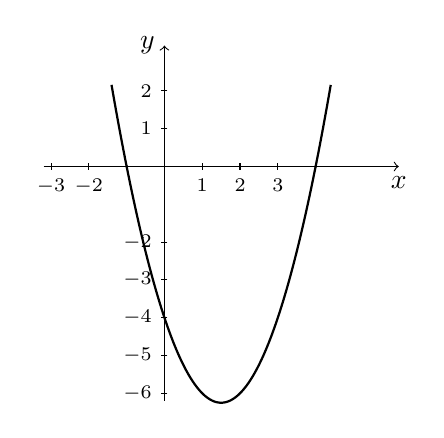
\begin{tikzpicture}[scale=0.48]
    \draw[->] (-3.2,0) -- (6.2,0) node[below] {$x$};
    \draw[->] (0,-6.2) -- (0,3.2) node[left] {$y$};
    \foreach \x in {-3,-2,1,2,3}
      \draw (\x,0.08)--(\x,-0.08) node[below] {\scriptsize $\x$};
    \foreach \y in {-6,-5,-4,-3,-2,1,2}
      \draw (0.08,\y)--(-0.08,\y) node[left] {\scriptsize $\y$};
    \draw[smooth, samples=200, domain=-1.4:4.4, thick] plot (\x, {\x*\x-3*\x-4});
    \fill (-1,0) circle (1.2pt);
    \fill (4,0) circle (1.2pt);
\end{tikzpicture}
